\section{Tsiligiridis' Algorithms}
\label{sec:03:tsiligiridis}

One of the earliest solution approaches for the \op{} was proposed by \citeauthor{tsiligiridis_heuristic_1984} in his 1984 paper on the topic \cite{tsiligiridis_heuristic_1984}.
He introduced two algorithms which generate a path and an algorithm that tries to improve an already existing path.

Only one of the two path-generating algorithms will be introduced here:
We will present the \emph{S-Algorithm} (see \cref{subsec:03:salgo}), since the \emph{D-Algorithm} requires a division of the plane into sections, which seems to have no trivial generalization to non-Euclidean inputs.
The route-improving \emph{R-I-Algorithm} will also be introduced (see \cref{subsec:03:rialgo}).
In his original paper, the input is assumed to be Euclidean but
we will discuss whether these algorithms can work on non-Euclidean inputs.

\subsection{Stochastic Algorithm}
\label{subsec:03:salgo}

The first algorithm described by \citeauthor{tsiligiridis_heuristic_1984} is the \emph{Stochastic Algorithm} (S-Algorithm).
It starts at the start node and iteratively constructs a path by randomly choosing an available node in each step.
They are not chosen \emph{uniformly} at random. Rather each node's probability of being chosen depend on a calculated desirability value which will be defined shortly.
If at any point, the only available node is the end node, it is chosen as the last node of the path and the algorithm terminates.

To recount, $G = (V, E)$ is a complete Euclidean graph with $n := |V|$.
$s(v_i)$ refers to the score of node $v_i \in V$, whereas $t(v_i,v_j)$ refers to the weight of the edge $\{v_i, v_j\}$ for $1 \leq i \neq j \leq n$.
$v_1 \in V$ is the start node and $v_n \in V$ the end node.
However there are some more variables required by this algorithm.

Let $last \in V$ refer to the last node visited by the algorithm in its previous step.
A node $v_i \in V$ is considered to be \emph{available} iff it has not been visited yet and adding it to the current path would not violate $T_{max}$ when adding the distances $t(last, v_i)$ and $t(v_i, v_n)$. (akin to the example in \cref{subsec:02:triangle}) 
The end node $v_n$ is excluded from this however.
Then let $A \subset V$ be the set of currently available nodes. 
Let $r \in \mathbb{R}_+$ be a parameter used to scale the desirability value exponentially.

Then the desirability value $D(v_i)$ for every $v_i \in A$ is defined as follows:

\begin{align*}
    D(v_i) := \left( \frac{s(v_i)}{t(last, v_i)} \right)^r
\end{align*}

This value aims to provide a measure for how valuable a node is estimated to be when included in the path.
The last parameter we will use is $1 \leq l \in \mathbb{N}$ which represents the maximum number of available nodes we want to consider in each iteration when choosing a node at random.
We only consider the $l$ most desirable nodes.

So to in short summarize the algorithm, we initialize the path with only $v_1$ and $A = V / \{v_1, v_n\}$.
We update $A$ by checking all nodes $v_i \in A$ whether adding $v_i$ would violate $T_{max}$ and removing those that do. 
We calculate all desirability values $D(v_i)$ for the remaining elements in $A$ and take the $k$ most desirable nodes from $A$ where $k := \min(l, |A|)$. Let $A'$ be the set of these nodes.
For each of these nodes $v_i \in A'$ the probability of being chosen is equal to:
\begin{align*}
    \frac{D(v_i)}{\sum_{j=1}^k D(v_j)}
\end{align*}
Choose a node according to these probabilities, insert it into the path and repeat the process (save for the initialization).

\begin{wrapfigure}{r}{5cm}
    \centering
    \scalebox{0.9}{
        \begin{tikzpicture}[vertex/.style={draw}]
            \node at (1, 2.2) {$T_{max}=4$};
            \node at (-1,0) (invis) {};
            \node[vertex, red] at (0,0) (0) {$0$};
            \node[vertex] at (2,0) (1) {$0$};
            \node[vertex, blue] at (1,1) (2) {$4$};
            \node[vertex, blue] at (1,-1) (3) {$6$};
            \node at (3,0) (invis2) {};

            \node[blue] at (1,1.6) {$\tfrac{4}{7}$};
            \node[blue] at (1,-1.6) {$\tfrac{3}{7}$};

            \draw[->, red] (invis) -- (0);
            \draw (0) -- node[above left] {$1$} (1);
            \draw[blue] (0) |- node [below right] {$1$} (2);
            \draw[blue] (0) |- node [above right] {$2$} (3);
            \draw (2) -- (3);
            \draw (2) -| node [below left] {$2$} (1);
            \draw (3) -| node [above left] {$2$} (1);
            \draw[->] (1) -- (invis2);
        \end{tikzpicture}
    }
    \caption{The S-Algorithm at work.}
    \label{fig:03:salgoexample}
\end{wrapfigure}

A small example is illustrated in \cref{fig:03:salgoexample}.
The number inside of a node is its score. 
The blue-colored nodes are available nodes that the algorithm is considering and the numbers besides the blue nodes are the probabilities of this node being chosen.
Elements that are currently part of the path are colored red.

There are other elements in these equations in the original paper not covered here.
However, as noted by \citeauthor{tsiligiridis_heuristic_1984}, these other values did not contribute to the quality of the solution in his evaluations, so they are omitted here. 

\subsubsection{Adapting for non-Euclidean inputs}

The inputs in \citeauthor{tsiligiridis_heuristic_1984}' paper are Euclidean and his descriptions are formulated in respect to a Euclidean input.
However the algorithm does not explicitly require the graph to have any particular properties except for every node to be directly connected to the end node $v_n$.
The reason for this is that the algorithm considers a node $v_i$ to be available if the path can move from the last visited node to $v_i$ and from $v_i$ to $v_n$ without violating $T_{max}$.

\begin{wrapfigure}{l}{5.5cm}
    \centering
    \scalebox{0.9}{
        \begin{tikzpicture}[vertex/.style={draw}]
            \node at (-1,0) (invis) {};
            \node[vertex] at (0,0) (0) {$v_0$};
            \node[below=0mm of 0] (w0) {$0$};
            \node[vertex] at (0,2) (1) {$v_1$};
            \node[above=0.5mm of 1] (w1) {$10$};
            \node[vertex] at (2,2) (2) {$v_2$};
            \node[above=0.5mm of 2] (w2) {$5$};
            \node[vertex] at (2,0) (3) {$v_3$};
            \node[below=0.5mm of 3] (w3) {$0$};
            \node at (3,0) (invis2) {};

            \draw[->] (invis) -- (0);
            \draw (0) -- node[left] {$1$} (1);
            \draw (1) -- node[above] {$1$} (2);
            \draw (2) -- node[right] {$1$} (3);
            \draw (0) -- node[below] {$5$} (3);
            \draw (0) -- node[left] {$3$} (2);
            \draw (1) -- (3);

            \draw[->] (3) -- (invis2);

            \node at (1, 3) {$T_{max}=3$};
        \end{tikzpicture}
    }
    \caption{An example that illustrates that the S-Algorithm can fail to find a path even in very simple graphs not fulfilling the triangle equation.}
    \label{fig:03:salgofailexample}
\end{wrapfigure}

As explained in \cref{subsec:02:triangle}, for this heuristic to work, the graph should satisfy the triangle inequality.
Otherwise it is not possible to decide whether a constraint-respecting path can be found when including this vertex; at least not in the way this algorithm does it.
If the graph does not satisfy the inequality, this might lead the algorithm to miss pursuing paths that might be profitable,
or might even lead to the algorithm not being able to find a path even in very small graphs. 

This is illustrated in \cref{fig:03:salgofailexample}. The obvious optimal path is the path taking all the edges with weight $1$.
However, $v_1$ has a weight $3$ edge to the end node and $v_2$ has a weight $3$ edge leading to it.
If any of these nodes were added to the path, they would lead to a path cost of $4$ (remember that we include the cost of the edge from $v_1$ or $v_2$ to the end node $v_3$), violating $T_{max} = 3$.
In addition, since the edge between the start and end node has a weight of $5$, this edge cannot be taken either.
As a result, the algorithm will not consider any nodes to be available and output that no path was found.
This result is obviously incorrect.

As alluded to before in \cref{subsec:02:complete}, one can make a graph complete by inserting missing edges with a weight of $\infty$.
This however, would violate the triangle inequality.
The algorithm would also ignore \emph{all} nodes $v_i$ with an $\infty$-edge to the end node $v_n$, since the edge $\{v_i, v_n\}$ could never be traversed, unless $T_{max} = \infty$.
But in this case there is no problem to solve.
One can easily imagine a graph with three nodes $A, B, C$ and edges $\{A, B\}$ and $\{B, C\}$, each having a respective finite weight $x$ and $y$.
If we were to complete this graph by inserting the edge $\{A, C\}$ with a weight of $\infty$, then $t(A, B) + t(B,C) = x + y < \infty = t(A, C)$
which is an obvious violation of the triangle inequality.

As a result, this algorithm can work correctly on complete graphs which satisfy the triangle inequality with none of its functionality being hampered.
However other graphs would likely result in sub-optimal results. 

%\subsection{Deterministic Algorithm}
\label{subsec:03:dalgo}

The second algorithm presented is the \emph{Deterministic Algorithm} (D-Algorithm).
This will only be briefly outlined for reasons explained later.

\begin{wrapfigure}{l}{0.5\textwidth}
    \centering
    \begin{tikzpicture}[pienode/.style 2 args={ circle, minimum size=#1, inner sep=0pt, path picture={\fill[red!30] (path picture
    bounding box.center) -- ++(0:#1) arc[start angle=0, end angle=3.6*#2,
    radius=#1] --cycle;}}]
        \node[pienode={4cm}{60}] (a) {};
        \node[circle,fill=white,minimum size=2cm] {};

        \node[draw,shape=circle,minimum width=4cm] at (0,0) (a) {};
        \node[draw,shape=circle,minimum width=2cm] at (0,0) (a) {};

        \draw (0,0) -- (0:2);
        \draw (0,0) -- (216:2);
        \draw[black!40] (0.3,0) arc[start angle=0, end angle=216, radius=3mm];

        \draw[-Circle] (170:1.2) -- (200:1.9);
        \draw[Circle-] (170:1.2) -- (160:1.7);
        \draw[-Circle] (160:1.7) -- (130:1.1);
        \draw[Circle-] (100:1.8) -- (130:1.1);
        \draw[-Circle] (100:1.8) -- (70:1.3);
        \draw[Circle-] (50:1.5) -- (70:1.3);
        \draw[-Circle] (50:1.5) -- (10:1.8);
    \end{tikzpicture}
    \caption{An example of the D-Algorithm creating a path restricted to a section.}
    \label{fig:03:dalgoexample}
\end{wrapfigure}

The D-Algorithm is inspired by \citeauthor{wren_computer_1972} and their algorithm for vehicle routing \cite{wren_computer_1972}.
Space is divided into different sections each given using concentric circles with different radii and an arc each.
An example of this is depicted in \cref{fig:03:dalgoexample}.
In \citeauthor{tsiligiridis_heuristic_1984} case, twelve different radii and arcs of $90\degree$ are used.
So space is divided into four quadrants, each being divided into $13$ segments.

A route is successively created for each sector, each route only using nodes that are in the respective sector.
This is done to reduce the travel distance from node to node.
In each sector, nodes are added until either no other node can be added due to violating $T_{max}$ or if all nodes of this sector have already been visited.

\subsubsection{Adapting for non-Euclidean Inputs}

As said before, this algorithm is only briefly explained.
The reason for this is that this algorithm cannot be easily generalized to non-Euclidean inputs.
This algorithm divides \emph{space} into sectors 
and using this terminology already hints at the fact that we need to measure and quantify \emph{space}, for example by using a metric.
And this leads us back to a Euclidean input.

Of course, the Euclidean metric is by far not the only one in existence.
One could possibly construct a similar division of the space by using a different metric, if a replacement for the concept of arcs and angles can be formulated.

Though, even under that assumption, this would shift the original problem to requiring another metric instead of the Euclidean one, 
in addition to finding adaptations and replacements for aspects of the algorithm that do not work when not using the Euclidean metric.
In addition, especially for real-world applications the Euclidean metric is by far the most prevalent and useful (see \cref{subsec:02:reasons}).
So not only would we be replacing the one problem with another, we would most likely be requiring an even rarer input due to requiring a more niche metric.
Needless to say, this would not be a generalization of this algorithm.

If not using a metric at all, one would need to partition the graph without the ability to use this metric. 
One would need to do away with the idea of sectioning space into sectors and instead divide the graph in another way.
This could perhaps be done using algorithms that allow dividing the graph into clusters, like Girvan and Newman's algorithm \cite{girvan_community_2002} which tries to identify edges connecting \emph{tightly-knit groups} and isolating those groups.
Though one would have to evaluate the quality of the solution with experiments.

In summary, there seems to be no trivial generalization of this algorithm to less restricted inputs.
\subsection{Route-Improvement Algorithm}
\label{subsec:03:rialgo}

The \emph{route-improvement algorithm} (R-I-Algorithm) does not generate a path.
Rather, it takes a pre-existing path as input and tries to improve upon it.
It therefore can be used in conjunction with any path-generating algorithm.
Improving paths is done using three methods.

\begin{enumerate}
	\itemsep0em
	\item Reorder nodes in the path.
	\item Introduce new nodes
	\item Replace one node with another.
\end{enumerate}

\iffalse
\begin{wrapfigure}{l}{0.45\textwidth}
	\centering
	\begin{subfigure}{0.45\textwidth}
		\centering
		\scalebox{0.78}{
			\begin{tikzpicture}[vertex/.style={draw}]
				\foreach \a in {1,...,6}{
						\draw (216-\a*360/10: 2.6cm) node (\a) {$v_\a$};
					}
				\draw[->] (1) -- (2);
				\draw[->] (2) -- (3);
				\draw[->] (3) -- (4);
				\draw[->] (4) -- (5);
				\draw[->] (5) -- (6);
			\end{tikzpicture}
		}
		\caption{A path generated by some algorithm.}
		\label{fig:03:rialgoreorderpath}
	\end{subfigure}
	\begin{subfigure}{0.45\textwidth}
		\centering
		\scalebox{0.78}{
			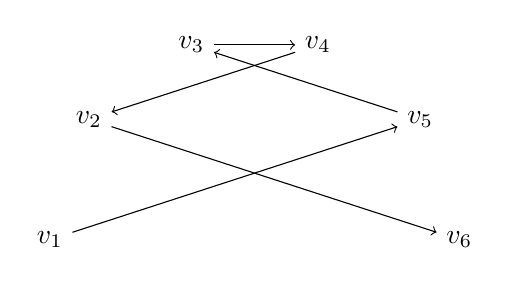
\begin{tikzpicture}[vertex/.style={draw}]
				\foreach \a in {1,...,6}{
						\draw (216-\a*360/10: 2.6cm) node (\a) {$v_\a$};
					}
				\draw[->] (1) -- (5);
				\draw[->] (5) -- (3);
				\draw[->] (3) -- (4);
				\draw[->] (4) -- (2);
				\draw[->] (2) -- (6);
			\end{tikzpicture}
		}
		\caption{Swapping $v_2$ and $v_5$, keeping the order of the nodes in between.}
		\label{fig:03:rialgoreorderkeep}
	\end{subfigure}
	\begin{subfigure}{0.45\textwidth}
		\centering
		\scalebox{0.78}{
			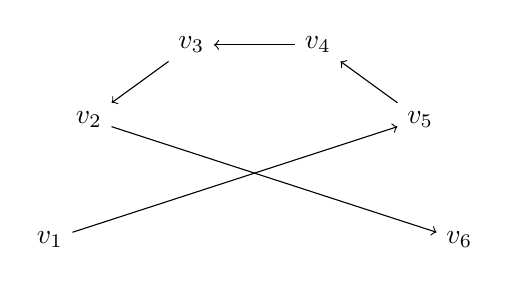
\begin{tikzpicture}[vertex/.style={draw}]
				\foreach \a in {1,...,6}{
						\draw (216-\a*360/10: 2.6cm) node (\a) {$v_\a$};
					}
				\draw[->] (1) -- (5);
				\draw[->] (5) -- (4);
				\draw[->] (4) -- (3);
				\draw[->] (3) -- (2);
				\draw[->] (2) -- (6);
			\end{tikzpicture}
		}
		\caption{Swapping $v_2$ and $v_5$, \emph{reversing} the order of the nodes in between.}
		\label{fig:03:rialgoreorderreverse}
	\end{subfigure}
	\caption{}
	\label{fig:03:rialgoreorder}
\end{wrapfigure}
\fi

\subsubsection{Reordering Nodes}
\label{subsubsec:03:reorder}

The first operation is to reorder nodes within a path by swapping two nodes.
While this will not increase a path's score, one hopes that it will reduce the path's total weight.

There are two types of swaps between two nodes $v_i$ and $v_j$.
\begin{enumerate}
	\itemsep0em
	\item Swap $v_i$ and $v_j$ keeping the order of nodes between them.
	\item Swap $v_i$ and $v_j$ and reverse the order of nodes between them.
\end{enumerate}
If any of the two types of swaps decreases the weight, the better swap is applied to the path.

Say the path is $v_1, v_2, v_3, v_4, v_5, v_6$.
If we swap nodes $v_2$ and $v_5$ and keep the order of the nodes in between them 
then the resulting path is $v_1, v_5, v_3, v_4, v_2, v_6$.
If instead we reverse the order of the nodes between $v_5$ and $v_2$, this results in the path $v_1, v_5, v_4, v_3, v_2, v_6$.

\subsubsection{Introduction of new Nodes}

In contrast to the previous section, this operation does not decrease the weight, but is only interested in increasing score.
Of course, only insertions that do not violate $T_{max}$ are allowed.
If a set of possible insertions is determined, the position that increases the cost the least is chosen.

\subsubsection{Replacing a Node}

This approach inserts an unvisited node into the path while at the same time removing another node from the path.
We choose a node $v_i$ which would be profitable to include in the path.
We then need to find the place in the path in which it would cause the smallest increase in the path's cost.
Then, find a node $v_j$ that if excluded would sufficiently decrease the cost of the path while minimizing the loss in score.
We can now remove $v_j$ from the path and insert $v_i$.
If there is a choice between multiple pairs of nodes, we pick the most profitable pair.

\subsubsection{Generalizing to non-Euclidean inputs}

Since this algorithm does not make any assumptions about its input, except for graph completeness it should work on any graph that is complete.



